\section{Dataset and Benchmark}
\label{sec:Dataset and Benchmark}

\paragraph{Revision-Derived Editing Supervision}
Our key observation is that plausible scientific figure edits naturally arise throughout scientific revision and development processes, including (i) figures modified across arXiv or GitHub versions, (ii) related (sub-)figures in the same paper or repository, (iii) alternative TikZ programs retained in source files but not rendered in the document, and (iv) iterative refinements in TeX SE discussions (Figure~\ref{fig:revision_sources}). Exact figure lineage is difficult to recover reliably as figures may be added, removed, renamed, reordered, or moved across files, while surrounding anchors such as captions, references, and related text can also change. We therefore identify semantically similar pairs within shared scientific contexts and retain plausible editing transformations.

\setkeys{Gin}{keepaspectratio}

\begin{figure*}[t]
\centering

\begin{tikzpicture}[
x=1cm,
y=1cm,
stage/.style={
    draw=gray!65,
    dashed,
    rounded corners=4pt,
    fill=gray!5,
    line width=0.3pt,
    inner sep=0pt
},
branch/.style={
    draw=gray!55,
    rounded corners=3pt,
    fill=white,
    line width=0.3pt,
    inner sep=0pt
},
paneltitle/.style={
    font=\bfseries\tiny,
    anchor=south west,
    inner sep=0pt
},
versionlabel/.style={
    font=\bfseries\tiny,
    anchor=south,
    inner sep=1pt
},
dots/.style={
    font=\bfseries\small,
    anchor=south,
    inner sep=1pt
},
img/.style={
    inner sep=0pt,
    outer sep=0pt,
    anchor=center
},
sourceimg/.style={
    draw=gray!45,
    line width=0.2pt,
    inner sep=0.1pt,
    outer sep=0pt,
    anchor=center
},
revision/.style={
    <->,
    >=stealth,
    line width=0.4pt
}
]

\node[
    stage,
    anchor=south west,
    minimum width=5.10cm,
    minimum height=2.65cm
] (stageone) at (0,0) {};

\node[paneltitle]
at ($(stageone.north west)+(0,0.04cm)$)
{1) Cross-Version Revisions};

\node[sourceimg] (paperone)
at ($(stageone.west)+(0.78cm,0)$) {%
    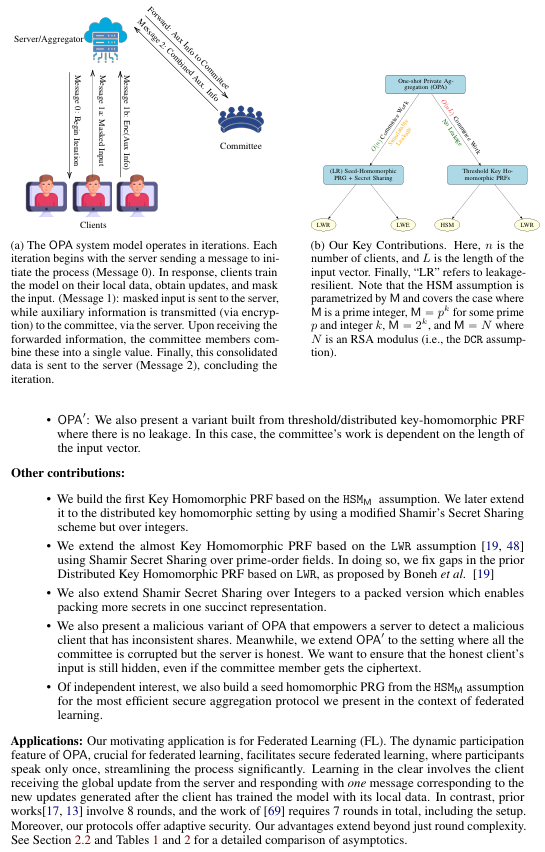
\includegraphics[
        width=2cm,
        height=2cm
    ]{structure/revision_figures/arxiv_diff_v1.png}%
};

\node[sourceimg] (papertwo)
at ($(paperone.east)+(0.95cm,0)$) {%
    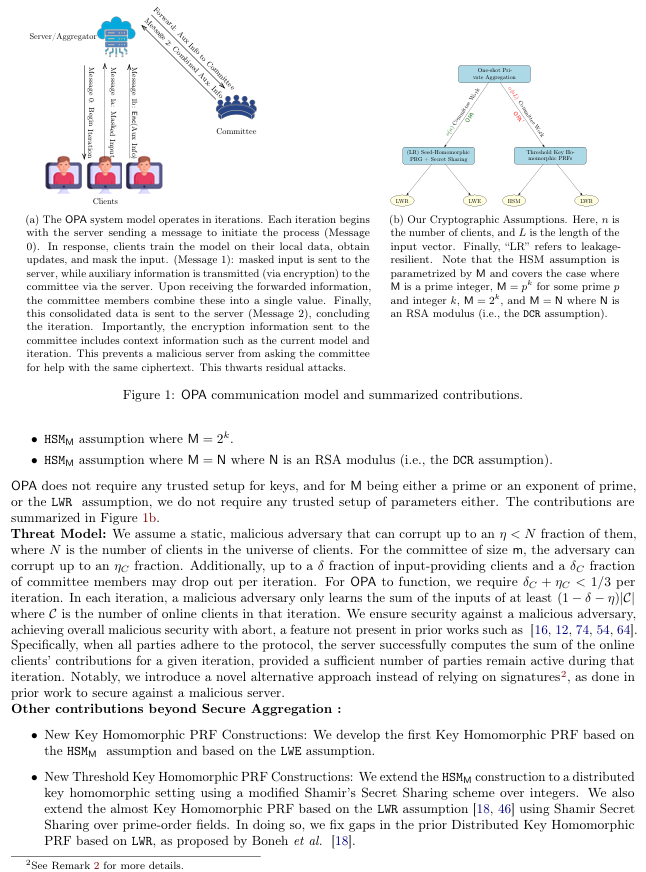
\includegraphics[
        width=2cm,
        height=2cm
    ]{structure/revision_figures/arxiv_diff_v3.png}%
};

\node[versionlabel]
at ($(paperone.north)+(0,0.0cm)$)
{$V_1$};

\node[versionlabel]
at ($(papertwo.north)+(0,0.0cm)$)
{$V_N$};

\node[dots]
at ($(paperone.east)+(0.105cm,-0.18cm)$)
{$\vdots$};

\node[
    branch,
    anchor=east,
    minimum width=1.50cm,
    minimum height=2.45cm
] (pairone)
at ($(stageone.east)+(-0.10cm,0)$) {};

\node[
    img,
    draw=red!85!black,
    line width=1.1pt
] (diffone)
at ($(pairone.center)+(0,0.70cm)$) {%
    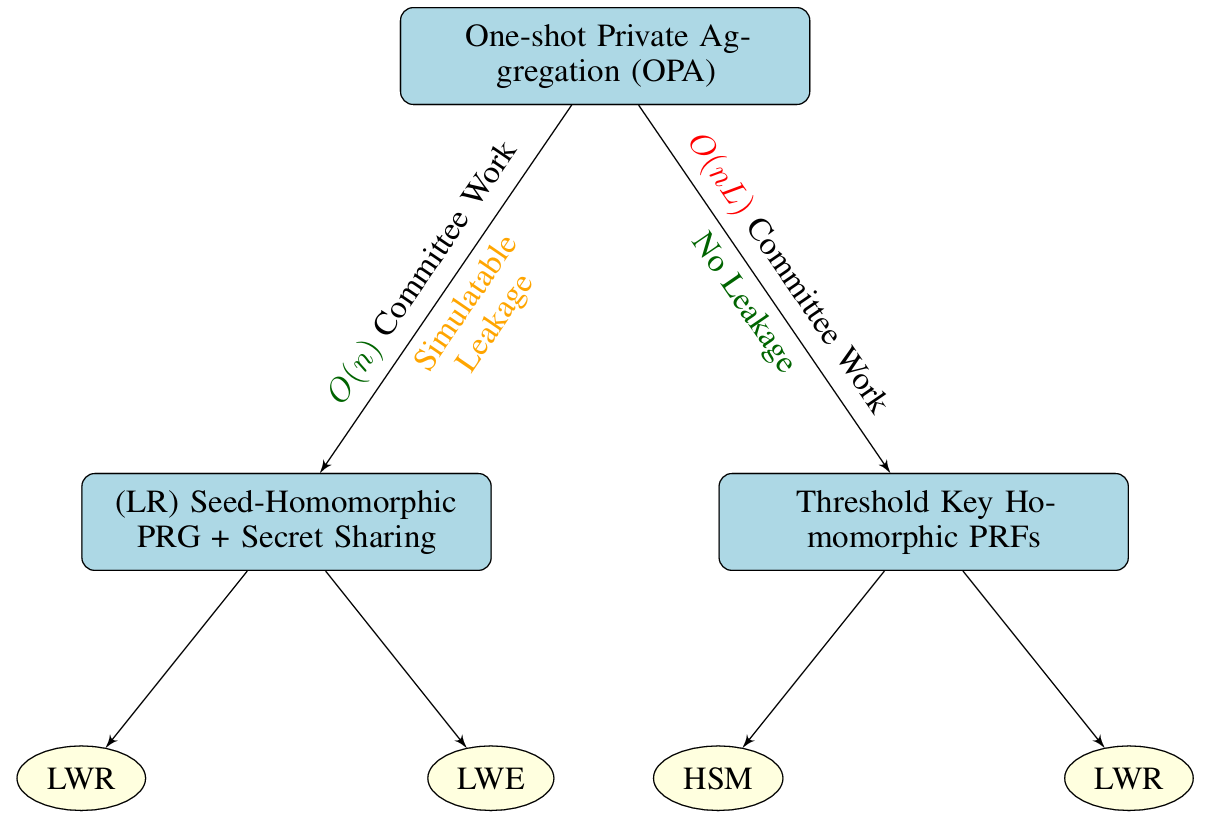
\includegraphics[
        width=1.4cm,
        height=1.4cm
    ]{structure/revision_figures/tikz_diff_v1.png}%
};

\node[
    img,
    draw=green!60!black,
    line width=1.1pt
] (difftwo)
at ($(pairone.center)+(0,-0.70cm)$) {%
    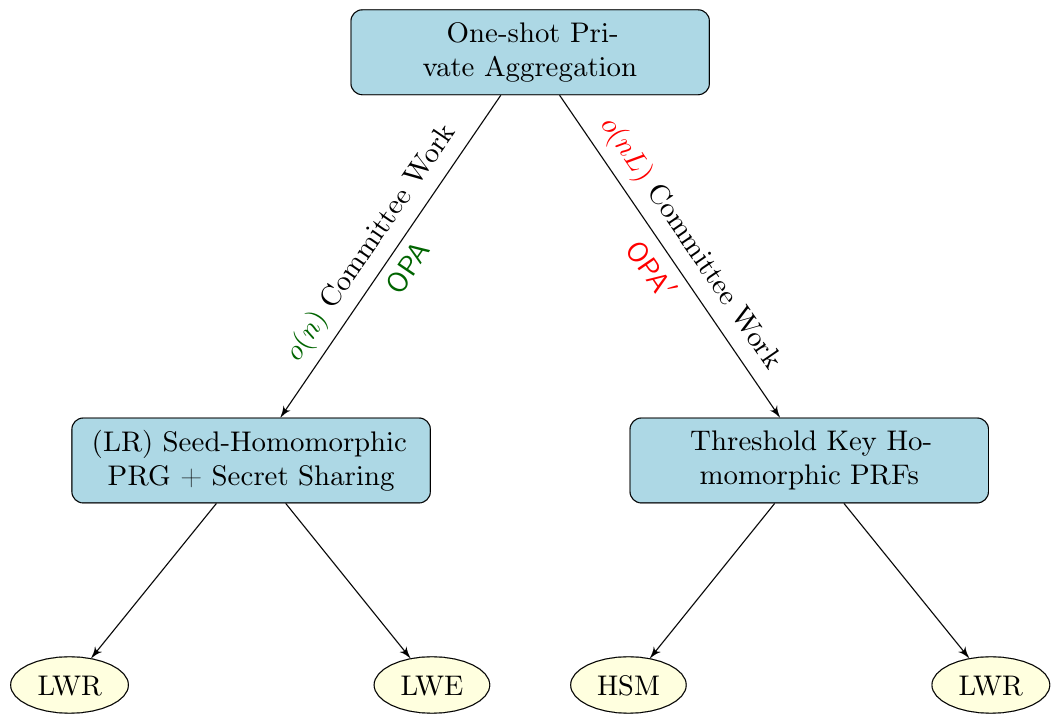
\includegraphics[
        width=1.4cm,
        height=1.4cm
    ]{structure/revision_figures/tikz_diff_v3.png}%
};

\draw[revision]
($(diffone.south)+(0,-0.03cm)$)
--
($(difftwo.north)+(0,0.03cm)$);

\coordinate (paperonefocus)
at ($(paperone.center)+(0.36cm,0.64cm)$);

\coordinate (papertwofocus)
at ($(papertwo.center)+(0.39cm,0.69cm)$);

\node[
    draw=red!85!black,
    line width=0.55pt,
    minimum width=0.55cm,
    minimum height=0.39cm,
    inner sep=0pt
] (paperonebox) at (paperonefocus) {};

\node[
    draw=green!60!black,
    line width=0.55pt,
    minimum width=0.50cm,
    minimum height=0.35cm,
    inner sep=0pt
] (papertwobox) at (papertwofocus) {};

\draw[
    red!85!black,
    ->,
    >=stealth,
    line width=0.55pt
]
(paperonebox.east)
to[out=20,in=150]
($(diffone.west)+(-0.01,0.0cm)$);

\draw[
    green!60!black,
    ->,
    >=stealth,
    line width=0.55pt
]
(papertwobox.east)
to[out=-20,in=150]
($(difftwo.west)+(-0.01,0.0cm)$);

\coordinate (redfocus)
at ($(diffone.center)+(-0.2cm,0.16cm)$);

\node[
    draw=red!85!black,
    line width=0.55pt,
    minimum width=0.27cm,
    minimum height=0.33cm,
    inner sep=0pt
] (redsource) at (redfocus) {};

\coordinate (redzoomcenter)
at ($(diffone.center)+(0.4125cm,0.121cm)$);

\begin{scope}
    \clip
        ($(redzoomcenter)+(-0.297cm,-0.363cm)$)
        rectangle
        ($(redzoomcenter)+(0.297cm,0.363cm)$);

    \node[inner sep=0pt]
    at ($(redzoomcenter)+(0.44cm,-0.352cm)$) {%
        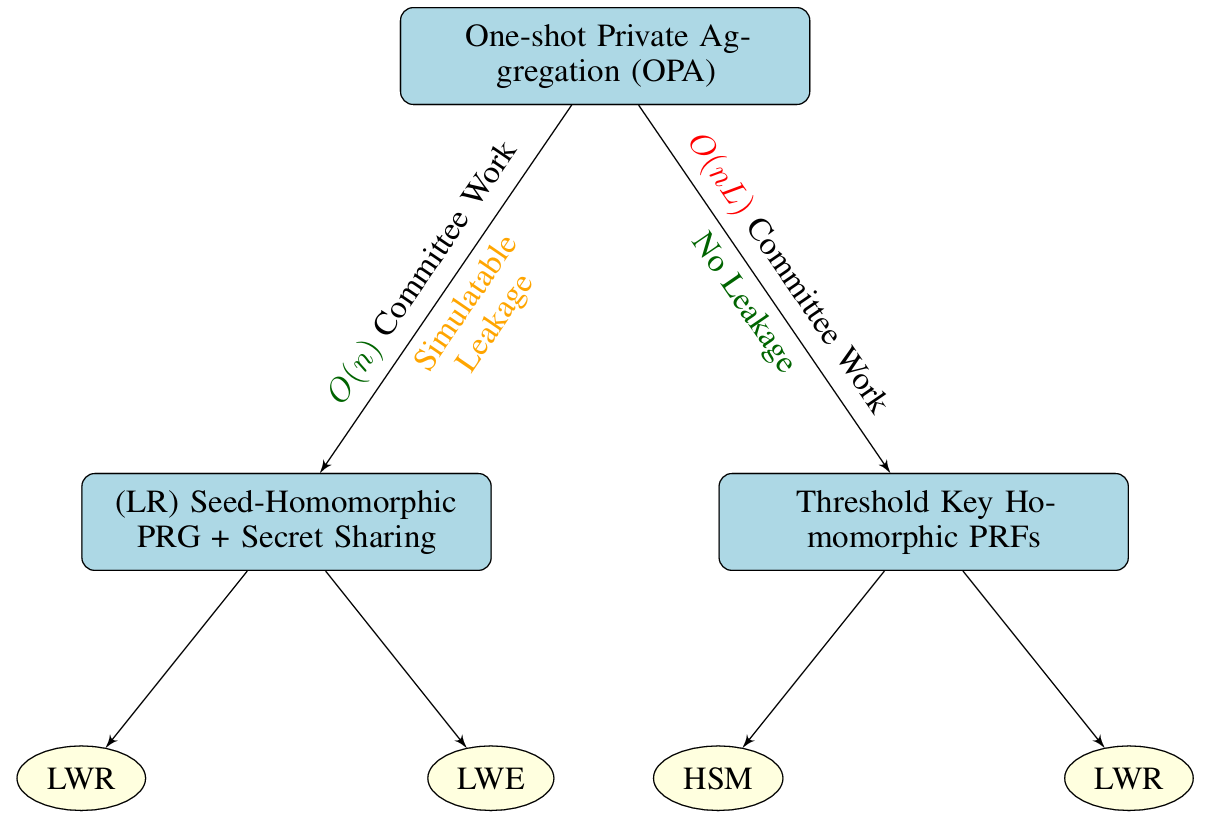
\includegraphics[
            width=3.08cm
        ]{structure/revision_figures/tikz_diff_v1.png}%
    };
\end{scope}

\draw[
    red!85!black,
    line width=0.55pt
]
($(redzoomcenter)+(-0.297cm,-0.363cm)$)
rectangle
($(redzoomcenter)+(0.297cm,0.363cm)$);

\draw[
    red!85!black,
    line width=0.45pt
]
(redsource.north east)
--
($(redzoomcenter)+(-0.297cm,0.363cm)$);

\draw[
    red!85!black,
    line width=0.45pt
]
(redsource.south east)
--
($(redzoomcenter)+(-0.297cm,-0.363cm)$);

\coordinate (greenfocus)
at ($(difftwo.center)+(-0.2cm,0.16cm)$);

\node[
    draw=green!60!black,
    line width=0.55pt,
    minimum width=0.27cm,
    minimum height=0.34cm,
    inner sep=0pt
] (greensource) at (greenfocus) {};

\coordinate (greenzoomcenter)
at ($(difftwo.center)+(0.4125cm,0.113cm)$);

\begin{scope}
    \clip
        ($(greenzoomcenter)+(-0.297cm,-0.374cm)$)
        rectangle
        ($(greenzoomcenter)+(0.297cm,0.374cm)$);

    \node[inner sep=0pt]
    at ($(greenzoomcenter)+(0.44cm,-0.352cm)$) {%
        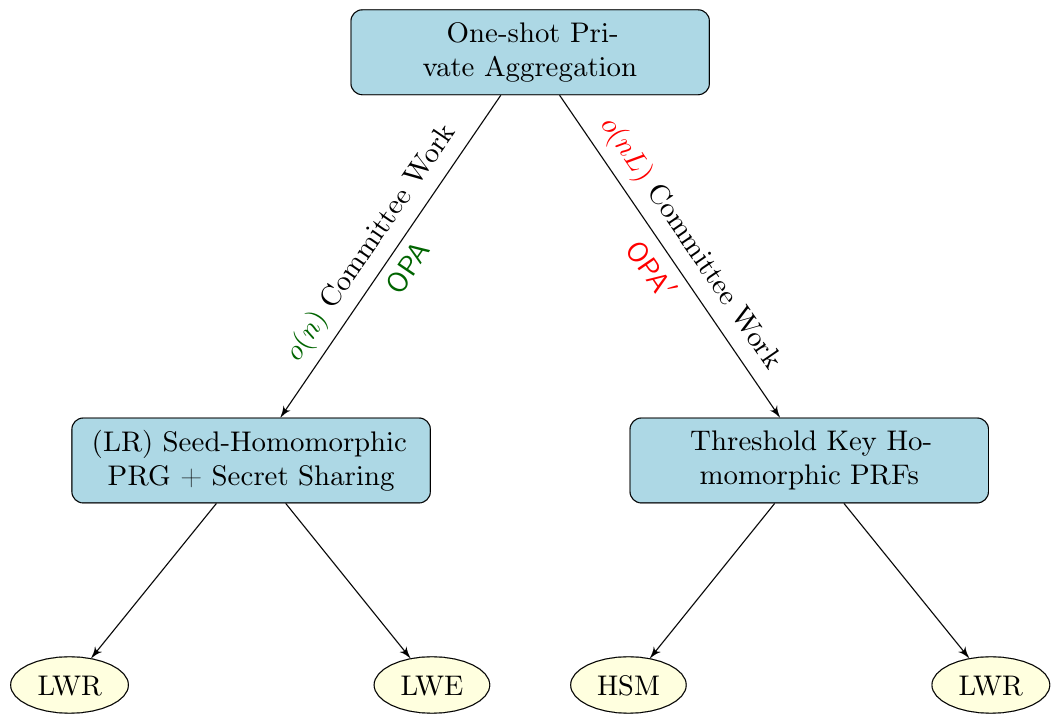
\includegraphics[
            width=3.08cm
        ]{structure/revision_figures/tikz_diff_v3.png}%
    };
\end{scope}

\draw[
    green!60!black,
    line width=0.55pt
]
($(greenzoomcenter)+(-0.297cm,-0.374cm)$)
rectangle
($(greenzoomcenter)+(0.297cm,0.374cm)$);

\draw[
    green!60!black,
    line width=0.45pt
]
(greensource.north east)
--
($(greenzoomcenter)+(-0.297cm,0.374cm)$);

\draw[
    green!60!black,
    line width=0.45pt
]
(greensource.south east)
--
($(greenzoomcenter)+(-0.297cm,-0.374cm)$);

\node[
    stage,
    anchor=south west,
    minimum width=4.75cm,
    minimum height=2.65cm
] (stagetwo)
at ($(stageone.south east)+(0.12cm,0)$) {};

\node[paneltitle]
at ($(stagetwo.north west)+(0,0.04cm)$)
{2) Related Figures/Subfigures};

\node[sourceimg] (subpaperone)
at ($(stagetwo.west)+(0.95cm,0.1cm)$) {%
    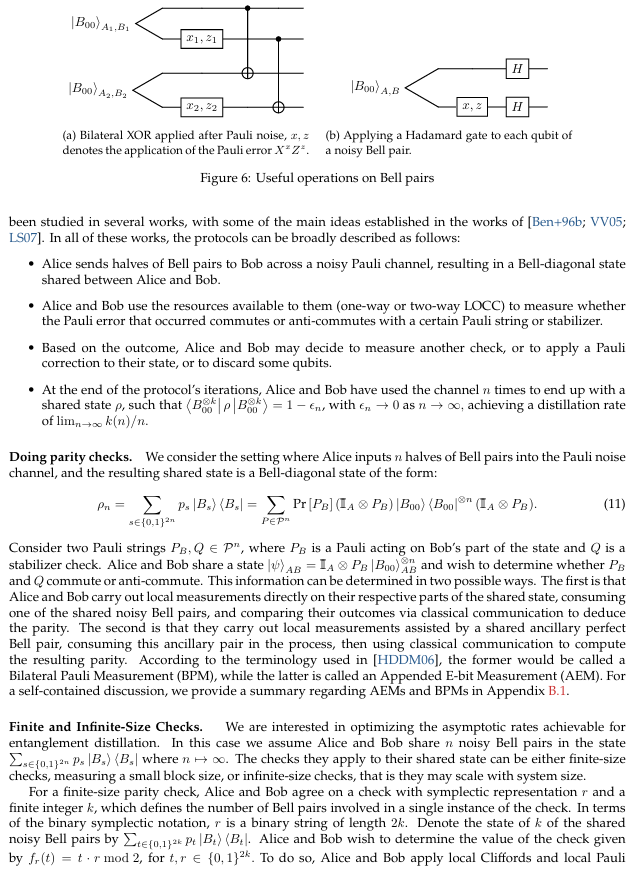
\includegraphics[
        width=2.2cm,
        height=2.2cm
    ]{structure/revision_figures/arxiv_subfigure_1.png}%
};

\node[sourceimg] (subpapertwo)
at ($(subpaperone.center)+(0.6cm,-0.2cm)$) {%
    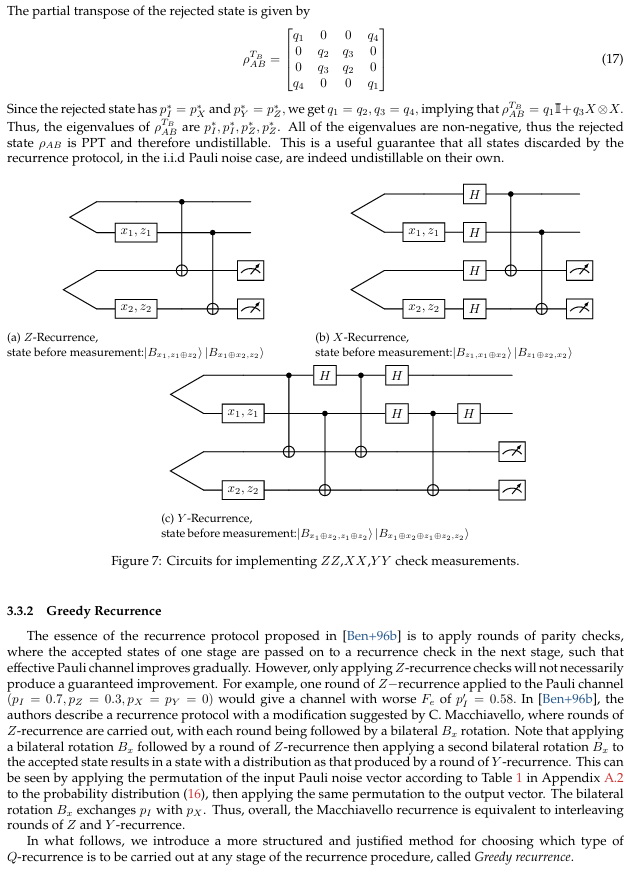
\includegraphics[
        width=2.2cm,
        height=2.2cm
    ]{structure/revision_figures/arxiv_subfigure_2.png}%
};

\node[
    branch,
    anchor=east,
    minimum width=1.9cm,
    minimum height=2.45cm
] (pairtwo)
at ($(stagetwo.east)+(-0.10cm,0)$) {};

\node[
    img,
    draw=red!85!black,
    line width=1.1pt
] (subone)
at ($(pairtwo.center)+(0,0.70cm)$) {%
    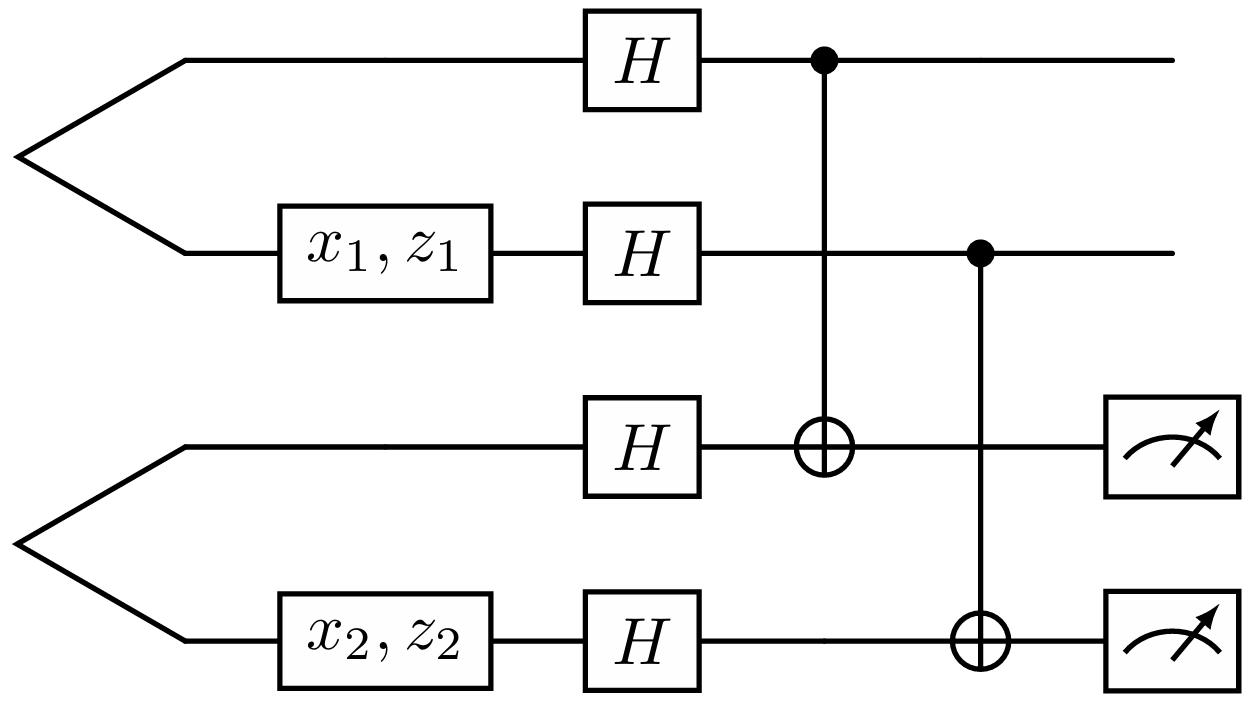
\includegraphics[
        width=1.7cm,
        height=1.7cm
    ]{structure/revision_figures/tikz_subfigure_4.png}%
};

\node[
    img,
    draw=green!60!black,
    line width=1.1pt
] (subtwo)
at ($(pairtwo.center)+(0,-0.70cm)$) {%
    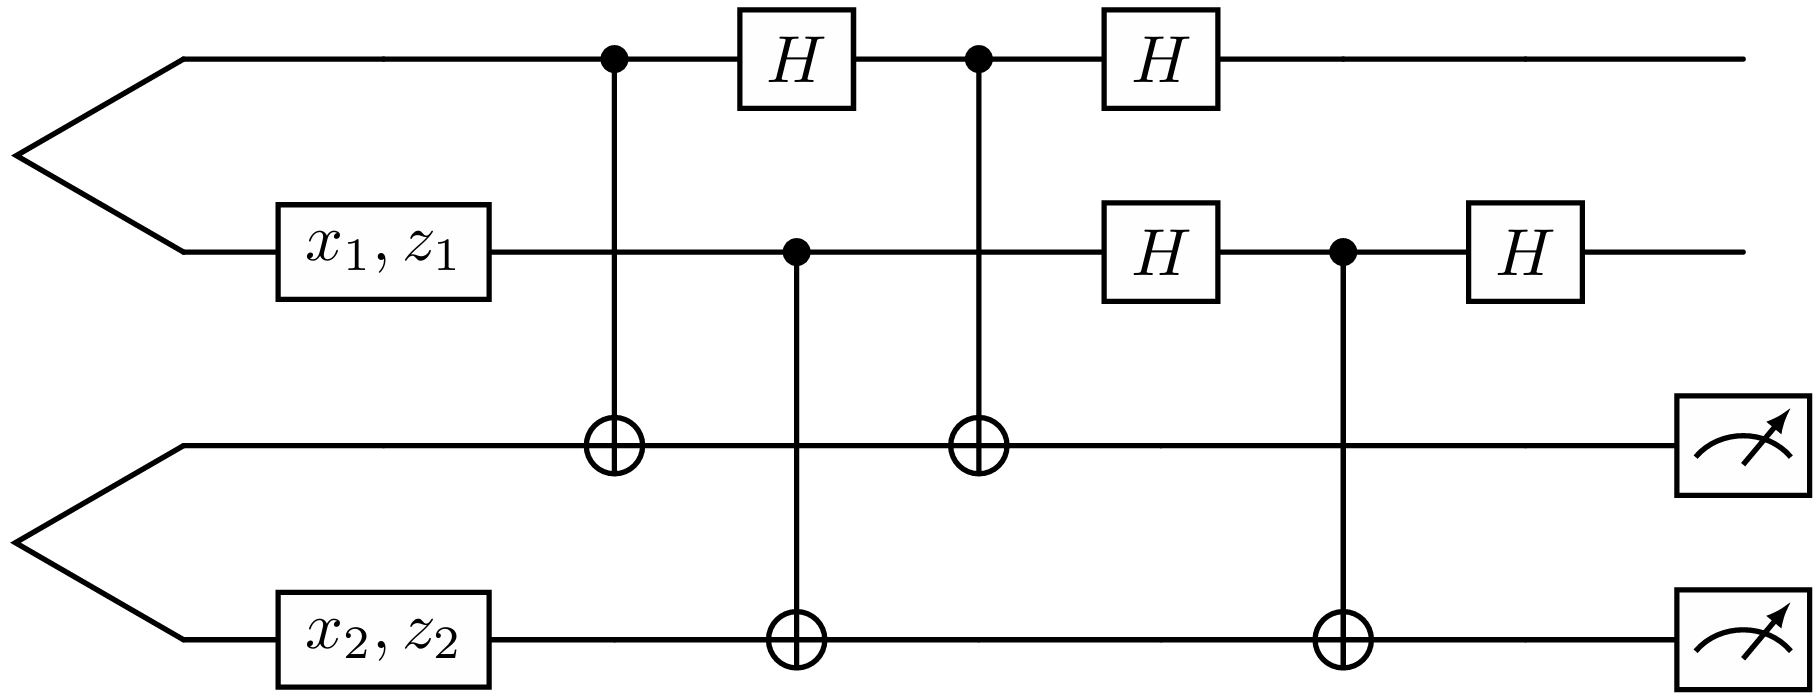
\includegraphics[
        width=1.7cm,
        height=1.7cm
    ]{structure/revision_figures/tikz_subfigure_5.png}%
};

\draw[revision]
($(subone.south)+(0,-0.03cm)$)
--
($(subtwo.north)+(0,0.03cm)$);

\coordinate (subpapertwopaironefocus)
at ($(subpapertwo.center)+(0.39cm,0.465cm)$);

\coordinate (subpapertwopairtwofocus)
at ($(subpapertwo.center)+(0.08cm,0.005cm)$);

\node[
    draw=red!85!black,
    line width=0.55pt,
    minimum width=0.645cm,
    minimum height=0.37cm,
    inner sep=0pt
] (subpapertwopaironebox) at (subpapertwopaironefocus) {};

\node[
    draw=green!60!black,
    line width=0.55pt,
    minimum width=0.93cm,
    minimum height=0.37cm,
    inner sep=0pt
] (subpapertwopairtwobox) at (subpapertwopairtwofocus) {};

\draw[
    red!85!black,
    ->,
    >=stealth,
    line width=0.55pt
]
(subpapertwopaironebox.east)
to[out=0,in=180]
($(subone.west)+(-0.01,0.0cm)$);

\draw[
    green!60!black,
    ->,
    >=stealth,
    line width=0.55pt
]
(subpapertwopairtwobox.east)
to[out=0,in=180]
($(subtwo.west)+(-0.01,0.0cm)$);

\node[
    stage,
    anchor=south west,
    minimum width=3.80cm,
    minimum height=2.65cm
] (stagethree)
at ($(stagetwo.south east)+(0.12cm,0)$) {};

\node[paneltitle]
at ($(stagethree.north west)+(0,0.04cm)$)
{3) TeX SE Discussions};

\node[sourceimg] (discussionone)
at ($(stagethree.west)+(0.8cm,0.12cm)$) {%
    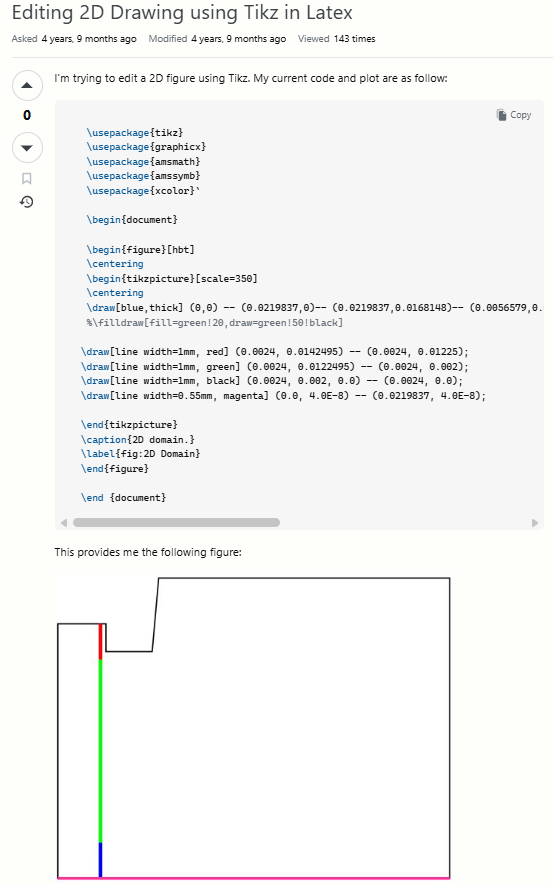
\includegraphics[
        width=2.2cm,
        height=2.2cm
    ]{structure/revision_figures/tex_discussion_1.png}%
};

\coordinate (discussiononefocus)
at ($(discussionone.center)+(0.0cm,-0.707cm)$);

\node[
    draw=red!85!black,
    line width=0.55pt,
    minimum width=1.15cm,
    minimum height=0.8cm,
    inner sep=0pt
] (discussiononebox) at (discussiononefocus) {};

\node[sourceimg] (discussiontwo)
at ($(discussionone.center)+(0.45cm,-0.24cm)$) {%
    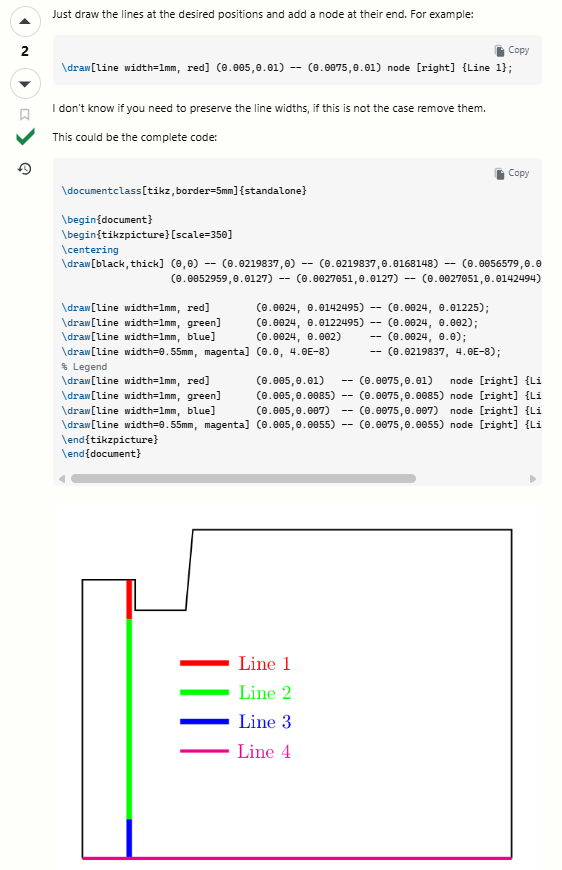
\includegraphics[
        width=2.2cm,
        height=2.2cm
    ]{structure/revision_figures/tex_discussion_3.png}%
};

\coordinate (discussiontwofocus)
at ($(discussiontwo.center)+(0.04cm,-0.655cm)$);

\node[
    draw=green!60!black,
    line width=0.55pt,
    minimum width=1.15cm,
    minimum height=0.88cm,
    inner sep=0pt
] (discussiontwobox) at (discussiontwofocus) {};

\node[
    branch,
    anchor=east,
    minimum width=1.34cm,
    minimum height=2.45cm
] (pairthree)
at ($(stagethree.east)+(-0.10cm,0)$) {};

\node[
    img,
    draw=red!85!black,
    line width=1.10pt
] (texone)
at ($(pairthree.center)+(0,0.70cm)$) {%
    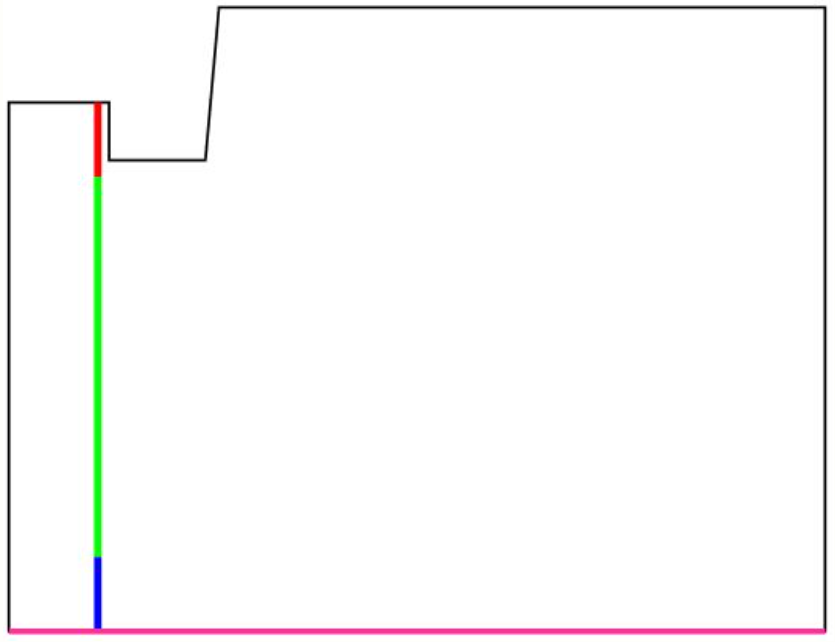
\includegraphics[
        width=1.2cm,
        height=1.2cm
    ]{structure/revision_figures/tex_tikz_1.png}%
};

\node[
    img,
    draw=green!60!black,
    line width=1.10pt
] (textwo)
at ($(pairthree.center)+(0,-0.70cm)$) {%
    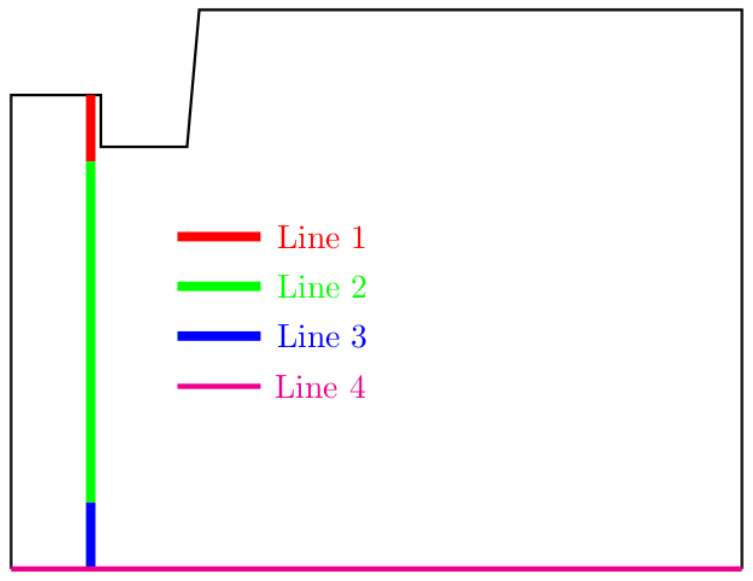
\includegraphics[
        width=1.2cm,
        height=1.2cm
    ]{structure/revision_figures/tex_tikz_2.png}%
};

\draw[revision]
($(texone.south)+(0,-0.03cm)$)
--
($(textwo.north)+(0,0.03cm)$);

\draw[
    red!85!black,
    ->,
    >=stealth,
    line width=0.55pt
]
($(discussiononebox.north)+(-0.40cm,0)$)
to[out=90,in=180]
($(texone.west)+(-0.01cm,0.0cm)$);

\draw[
    green!60!black,
    ->,
    >=stealth,
    line width=0.55pt
]
(discussiontwobox.east)
to[out=0,in=180]
($(textwo.west)+(-0.01,0.0cm)$);

\end{tikzpicture}

\caption{Sources of figure editing supervision. We recover plausible edit pairs from cross-version revisions (left), related figures and subfigures within shared scientific contexts (middle), and iterative refinements in TeX SE discussions (right). Red and green highlight paired variants in their sources.}
\label{fig:revision_sources}

\end{figure*}

\paragraph{Collecting Scientific Revision Traces}
We extend DaTikZ-V4~\citep{greisinger2026tikzilla} by recovering TikZ from all historical versions of arXiv submissions containing \texttt{tikzpicture}, \texttt{circuitikz}, or \texttt{tikzcd}. We apply the TikZilla preprocessing pipeline, including document expansion, subfigure extraction, code standardization, dynamic package inclusion, filtering, rendering, and deduplication on the standardized TikZ body. Across 91K arXiv submissions, 38K contain at least two versions with modified TikZ code. Historical versions contribute 0.77M additional figures, increasing the unique arXiv corpus from 1.47M to 2.38M. Combined with GitHub and TeX SE, this yields a candidate corpus of 2.91M unique TikZ figures.

\paragraph{Recovering Plausible Edit Pairs}
We group figures by arXiv submission across versions, GitHub repository, and TeX SE discussion thread, yielding 222K groups, of which 123K contain at least two unique figures. We prune groups above the 90th size percentile and compute within-group cosine similarities using \texttt{DeTikZify-V2}'s image encoder. To determine the filtering threshold, we manually evaluate 50 pairs in each of eight similarity intervals (0.92--0.9999, width 0.01) and retain intervals containing fewer than 15\% implausible transformations (Table~\ref{tab:semantic_similarity_examples}). This produces 430,442 candidate pairs from 87,051 contributing groups, connecting 589,986 unique figures.

\newlength{\simblockwidth}
\setlength{\simblockwidth}{0.238\textwidth}

\newlength{\simimagewidth}
\setlength{\simimagewidth}{0.108\textwidth}

\newlength{\simimageheight}
\setlength{\simimageheight}{1.65cm}

\newcommand{\simimage}[1]{%
  \begin{minipage}[c][\simimageheight][c]{\simimagewidth}
    \centering
    \includegraphics[
      width=\linewidth,
      height=0.94\simimageheight,
      keepaspectratio
    ]{#1}%
  \end{minipage}%
}

\newcommand{\simrange}[1]{%
  \fontsize{8}{9}\selectfont
  \textbf{#1}%
}

\newcommand{\simsubheader}[1]{%
  \fontsize{7}{8}\selectfont
  \textbf{#1}%
}

\newcommand{\similarityblock}[5]{%
  \begin{tikzpicture}[
    remember picture,
    baseline=(#1.base)
  ]
    \node[
      name=#1,
      anchor=center,
      inner xsep=2pt,
      inner ysep=3pt,
      outer sep=0pt,
      fill=#2,
      minimum width=\simblockwidth
    ]{%
      \begin{minipage}{\dimexpr\simblockwidth-4pt\relax}
        \centering

        \simrange{#3}

        \vspace{-5.5pt}
        \rule{\linewidth}{0.4pt}
        \vspace{-9pt}

        \begin{tabular}{@{}cc@{}}
          \simimage{#4} &
          \simimage{#5}
        \end{tabular}

        \vspace{-2pt}
      \end{minipage}%
    };
  \end{tikzpicture}%
}

\begin{table*}[t]
  \centering
  \caption{Examples of scientific-figure edit pairs across semantic-similarity intervals and the percentage of implausible editing transformations in each interval. Gray cells denote excluded intervals.}
  \label{tab:semantic_similarity_examples}

  \setlength{\tabcolsep}{2pt}
  \renewcommand{\arraystretch}{1}

  \begin{tabular}{@{}cccc@{}}
    \toprule
    \similarityblock
      {simtopone}
      {black!10}
      {$\boldsymbol{0.92\text{--}0.93}$ $\boldsymbol{(28\%)}$}
      {structure/similarities/sim_092_1.png}
      {structure/similarities/sim_092_2.png}
    &
    \similarityblock
      {simtoptwo}
      {black!10}
      {$\boldsymbol{0.94\text{--}0.95}$ $\boldsymbol{(18\%)}$}
      {structure/similarities/sim_094_1.png}
      {structure/similarities/sim_094_2.png}
    &
    \similarityblock
      {simtopthree}
      {white}
      {$\boldsymbol{0.96\text{--}0.97}$ $\boldsymbol{(8\%)}$}
      {structure/similarities/sim_096_1.png}
      {structure/similarities/sim_096_2.png}
    &
    \similarityblock
      {simtopfour}
      {white}
      {$\boldsymbol{0.98\text{--}0.99}$ $\boldsymbol{(2\%)}$}
      {structure/similarities/sim_098_1.png}
      {structure/similarities/sim_098_2.png}
    \\[4pt]
    \midrule
    \similarityblock
      {simbottomone}
      {black!10}
      {$\boldsymbol{0.93\text{--}0.94}$ $\boldsymbol{(22\%)}$}
      {structure/similarities/sim_093_1.png}
      {structure/similarities/sim_093_2.png}
    &
    \similarityblock
      {simbottomtwo}
      {white}
      {$\boldsymbol{0.95\text{--}0.96}$ $\boldsymbol{(10\%)}$}
      {structure/similarities/sim_095_1.png}
      {structure/similarities/sim_095_2.png}
    &
    \similarityblock
      {simbottomthree}
      {white}
      {$\boldsymbol{0.97\text{--}0.98}$ $\boldsymbol{(6\%)}$}
      {structure/similarities/sim_097_1.png}
      {structure/similarities/sim_097_2.png}
    &
    \similarityblock
      {simbottomfour}
      {white}
      {$\boldsymbol{0.99\text{--}0.9999}$ $\boldsymbol{(12\%)}$}
      {structure/similarities/sim_099_1_new.png}
      {structure/similarities/sim_099_2_new.png} 
    \\[4pt]
    \bottomrule
  \end{tabular}
\end{table*}

\paragraph{Inferring Edit Instructions}
Because both endpoint figures are human-authored, we synthesize only the missing edit instruction using Qwen3.6-27B conditioned jointly on their renders and TikZ code. For each of the 430,442 candidate pairs, we infer both directions ($A\!\rightarrow\!B$ and $B\!\rightarrow\!A$), producing 860,884 candidate directional trajectories. The VLM classifies each direction as \texttt{ok}, \texttt{invalid}, or \texttt{identical}. For accepted transformations, it decomposes the transformation into atomic edits with an intent (\texttt{add}, \texttt{remove}, or \texttt{modify}), operation (\texttt{text}, \texttt{annotation}, \texttt{geometry}, \texttt{data}, \texttt{style}, or \texttt{structure}), and natural-language description. Requiring both directions to be accepted yields DaEdiTikZ with 390,516 figure pairs and 781,032 directional editing trajectories. Each trajectory contains 4.2 atomic edits on average, with descriptions averaging 22.3 words per atomic edit. Detailed analysis of DaEdiTikZ is in the Appendix~\ref{subsec:Dataset and Benchmark}.

\newcommand{\smathn}[1]{\scalebox{0.45}{$#1$}}

\begin{figure*}[t]
\centering

\begin{adjustbox}{max width=\textwidth}
\begin{tikzpicture}[
  ampersand replacement=\&,
  >=Latex,
  node distance=0.45cm and 0.55cm,
  pipelinearrow/.style={
    -{Latex[length=2.5mm,width=1.8mm]},
    line width=0.9pt,
    draw=black
  },
  newlabel/.style={
    font=\sffamily\bfseries\LARGE,
    text=red,
    anchor=south,
    inner sep=1pt
  },
  arxivlabel/.style={
    font=\tiny,
    text=red,
    anchor=south,
    inner sep=1pt
  },
  pipelinethinarrow/.style={
    -{Latex[length=2.1mm,width=1.5mm]},
    line width=0.7pt,
    draw=black
  },
  process/.style={
    draw=black!75,
    line width=0.7pt,
    rounded corners=1pt,
    fill=orange!7,
    inner sep=5pt,
    align=left
  },
  logo/.style={
    draw=black!70,
    rectangle,
    rounded corners=3pt,
    fill=blue!4,
    minimum width=0.5cm,
    minimum height=0.8cm,
    inner sep=2pt,
    align=center
  },
  imagebox/.style={
    draw=black!65,
    line width=0.5pt,
    fill=white,
    inner sep=1.5pt
  },
  tablebox/.style={
    draw=none,
    fill=white,
    inner sep=0pt,
    outer sep=0pt,
    minimum width=0pt,
    minimum height=0pt,
    align=center
},
  pairbox/.style={
    draw=black!75,
    line width=0.7pt,
    fill=white,
    inner sep=1.5pt,
    outer sep=0pt,
    align=center
},
  llm/.style={
    draw=black!75,
    line width=0.7pt,
    fill=orange!7,
    inner sep=5pt,
    align=left
},
  instruction/.style={
    draw=black!75,
    line width=0.7pt,
    fill=orange!4,
    inner sep=3pt,
    align=left
},
  imageencoder/.style={
    draw=black!80,
    line width=0.8pt,
    trapezium,
    trapezium left angle=70,
    trapezium right angle=70,
    shape border rotate=270,
    minimum width=1.1cm,
    minimum height=0.8cm,
    fill=blue!10,
    align=center
}
]

\node[logo] (arxiv) at (0,0) {%
    
\includegraphics[width=1.00cm]{structure/logos/arxiv-logo.png}
};

\node[logo, right=0.055cm of arxiv] (github) {%
    
\includegraphics[width=0.6cm]{structure/logos/github-mark.png}
};

\node[logo, right=0.055cm of github] (tex) {%
    
\includegraphics[width=1.00cm]{structure/logos/se-logo.png}
};

\node[
    process,
    below=0.45cm of github,
    text width=2.66cm,
    align=left
] (filter) {
    \small
    \textbf{Data Preprocessing}\\
    \vspace{0.2em}
    \scriptsize
    \textbullet\ TikZilla Filtering \\
    \textbullet\ Rendering \\
    \textbullet\ Grouping \\
    \vspace{-0.55em}
    \textbullet\ Pruning
};

\node[
    anchor=north east,
    inner sep=0pt
] at ($(filter.north east)+(0.0cm,-1.3cm)$) {%
    
\includegraphics[width=0.5cm]{structure/logos/filter.png}
};

\draw[pipelinethinarrow]
    (arxiv.south) -- ++(0,-0.20)
    -| ($(filter.north west)+(0.42cm,0)$);

\draw[pipelinethinarrow]
    (github.south) -- ($(filter.north)+(0,0)$);

\draw[pipelinethinarrow]
    (tex.south) -- ++(0,-0.20)
    -| ($(filter.north east)+(-0.42cm,0)$);

\node[imagebox, anchor=north west] (pathone)
    at (3.5,0.13) {%
        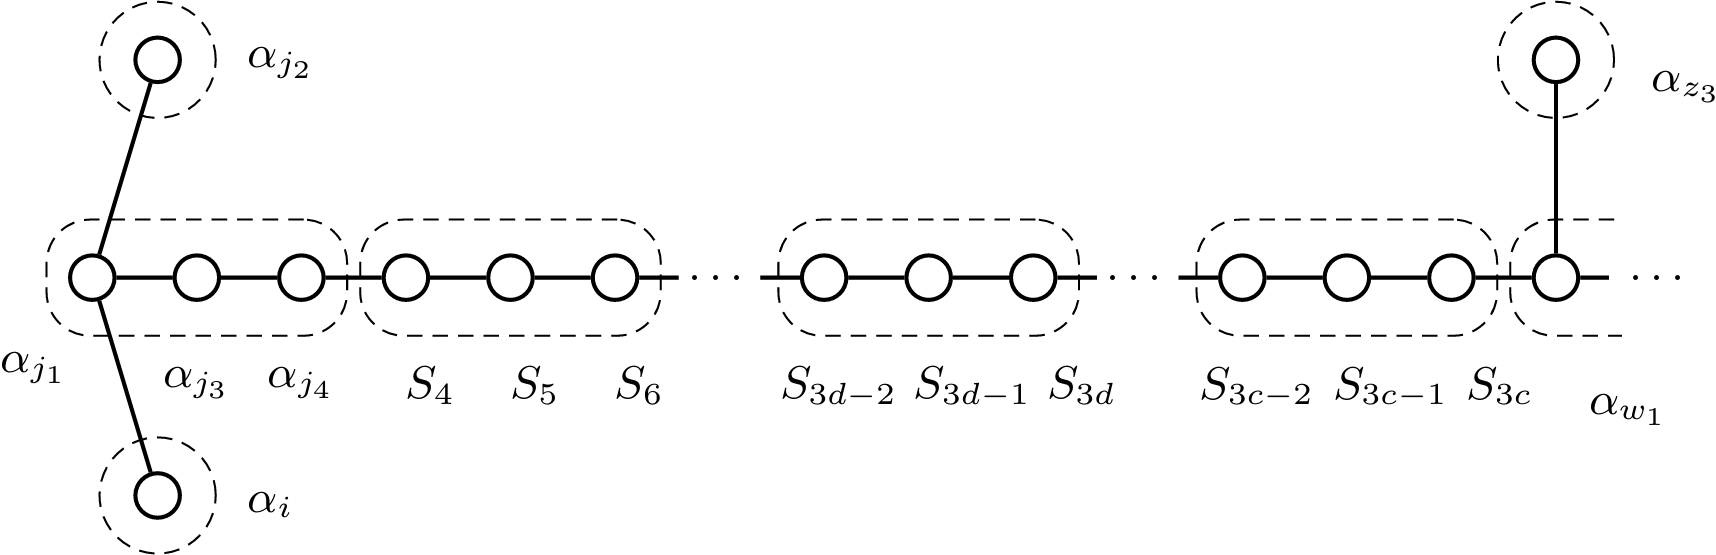
\includegraphics[
            width=1.5cm,
            height=0.5cm,
            keepaspectratio
        ]{structure/figures_dataset/structure_1.png}
    };

\node[imagebox, anchor=north west] (pathtwo)
    at (4.2,-0.5) {%
        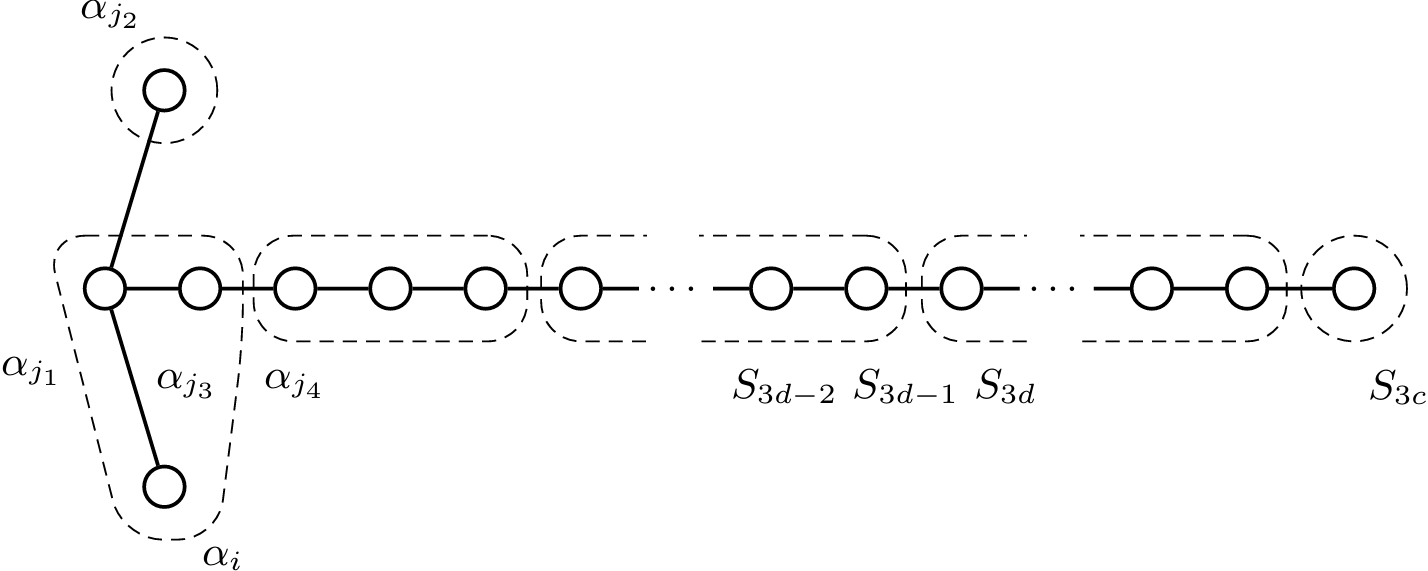
\includegraphics[
            width=1.5cm,
            height=0.5cm,
            keepaspectratio
        ]{structure/figures_dataset/structure_2.png}
    };

\node[imagebox, anchor=north west] (heatmap)
    at (4.2,-1.15) {%
        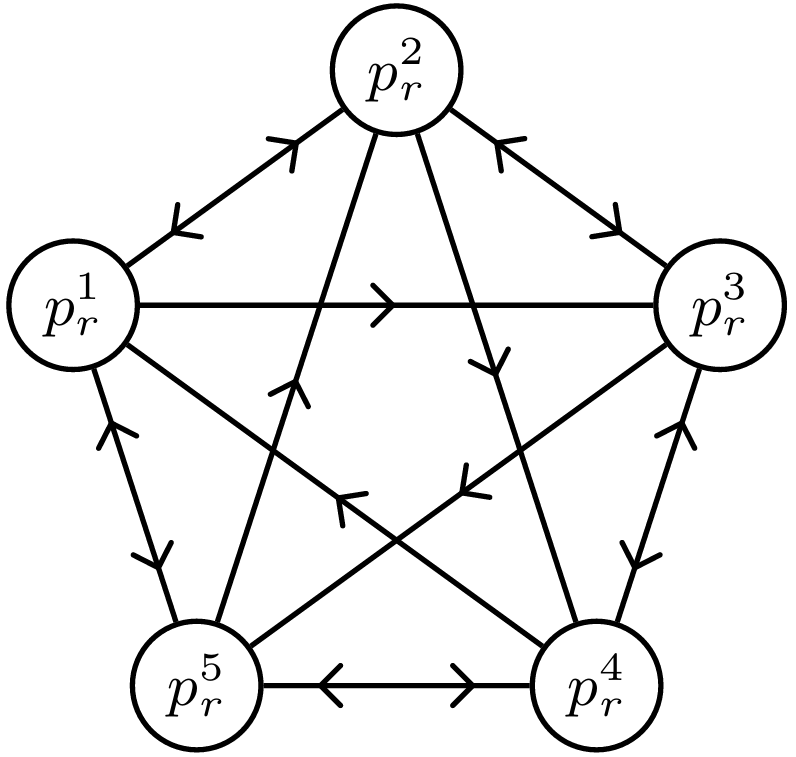
\includegraphics[
            width=0.95cm,
            height=0.95cm,
            keepaspectratio
        ]{structure/figures_dataset/penta_path.png}
    };

\node[imagebox, anchor=north west] (verticalchart)
    at (3.0,-0.5) {%
        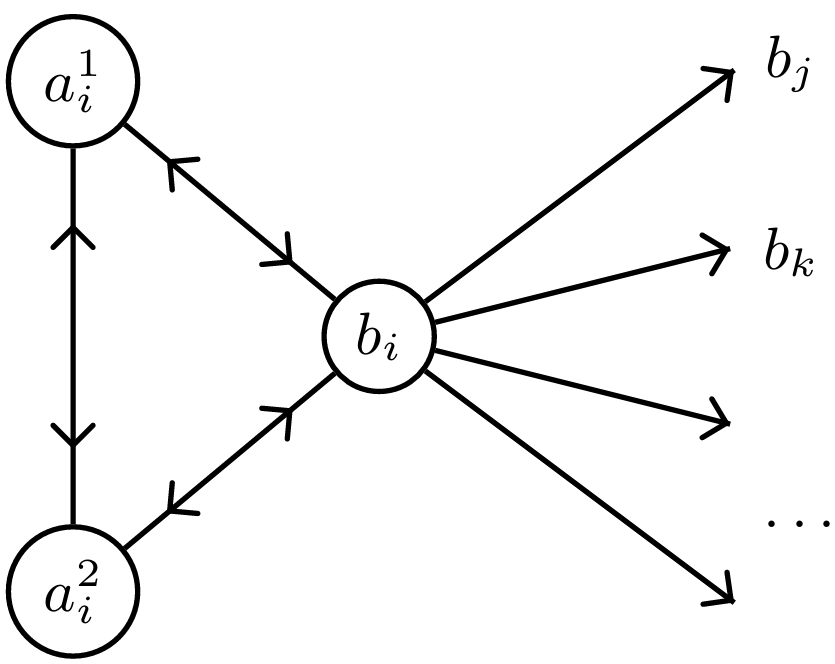
\includegraphics[
            width=1.05cm,
            height=1.05cm,
            keepaspectratio
        ]{structure/figures_dataset/path_node_edge.png}
    };

\node[newlabel] at (3.7,-2.0) {...};

\node[arxivlabel] at (4.3,-2.4) {arxiv/2107.04368};

\draw[pipelinethinarrow]
    (filter.east) to +($(0.33cm,0)$);

\draw[
  red,
  line width=1pt,
  dash pattern=on 5pt off 4pt
]
  (4.3,-1.10)
  ellipse [x radius=1.5cm,y radius=1.5cm];

\node[
    imageencoder,
    anchor=center
] (encoder) at (6.76,-0.2) {%
    \footnotesize IE
};

\node[
    tablebox,
    below=0.6cm of encoder
] (embmatrix) {%
{
\fontsize{3}{3.5}\selectfont
\setlength{\tabcolsep}{0.0pt}
\renewcommand{\arraystretch}{1.5}
\begin{tabular}{ccc}
\toprule
$\mathbf{e_1}$ & $\cdots$ & $\mathbf{e_N}$\\
\midrule
$-0.45$ & $\cdots$ & $0.52$\\
$0.03$ & $\cdots$ & $-0.01$\\
$0.27$ & $\cdots$ & $-0.79$\\[-2em]
$\vdots$ & $\ddots$ & $\vdots$\\
$0.82$ & $\cdots$ & $0.21$\\
\bottomrule
\end{tabular}
}
};

\draw[pipelinearrow]
    (encoder.south) -- ++(0.0,-0.6cm);

\draw[pipelinearrow]
    (5.5cm,-0.2cm) -- (encoder.west);

\node[
    tablebox,
    right=0.15cm of embmatrix,
    yshift=-0.1cm
] (simmatrix) {%
{
\fontsize{3}{3.5}\selectfont
\setlength{\tabcolsep}{0.7pt}
\renewcommand{\arraystretch}{1.15}
\begin{tabular}{c|cccc}
    & $\mathbf{i_1}$ & $\mathbf{i_2}$ & $\cdots$ & $\mathbf{i_N}$\\
\midrule
$\mathbf{i_1}$
    & $1.00$ & \textcolor{blue}{$0.98$} & $\cdots$ & \textcolor{red}{$0.92$}\\
$\mathbf{i_2}$
    & \textcolor{blue}{$0.98$} & $1.00$ & $\cdots$ & \textcolor{red}{$0.86$}\\[-2em]
$\vdots$
    & $\vdots$ & $\vdots$ & $\ddots$ & $\vdots$\\
$\mathbf{i_N}$
    & \textcolor{red}{$0.92$} & \textcolor{red}{$0.86$} & $\cdots$ & $1.00$\\
\end{tabular}
}
};

\draw[pipelinearrow]
    ($(embmatrix.east)+(-0.1,0)$)
    -- ++(0.4,0);

\node[
    pairbox,
    above=0.35cm of simmatrix
] (retainedpair) {%
    \begin{minipage}{1.9cm}
        \centering
        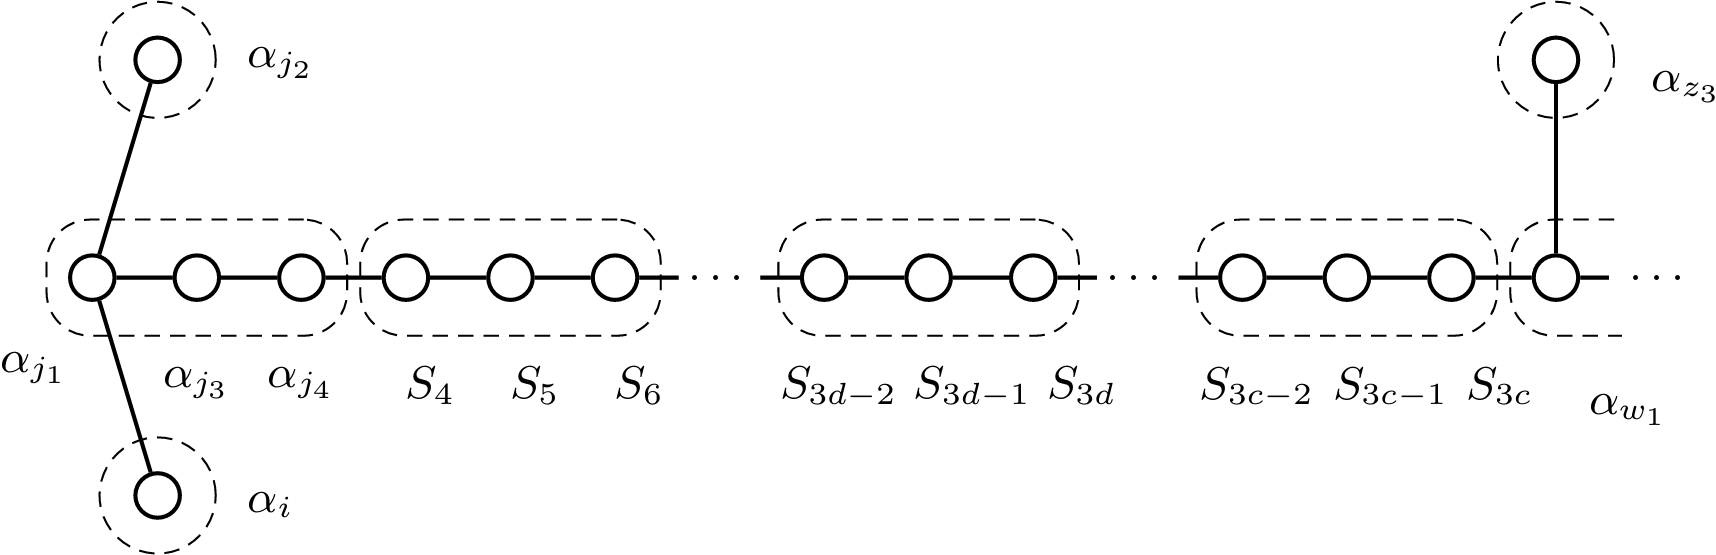
\includegraphics[
            width=2cm,
            height=0.75cm,
            keepaspectratio
        ]{structure/figures_dataset/structure_1.png}
        \\[-1.0em]
        \hspace*{0.6mm}\rule{1.85cm}{0.45pt}
        \\%[-0.15em]
        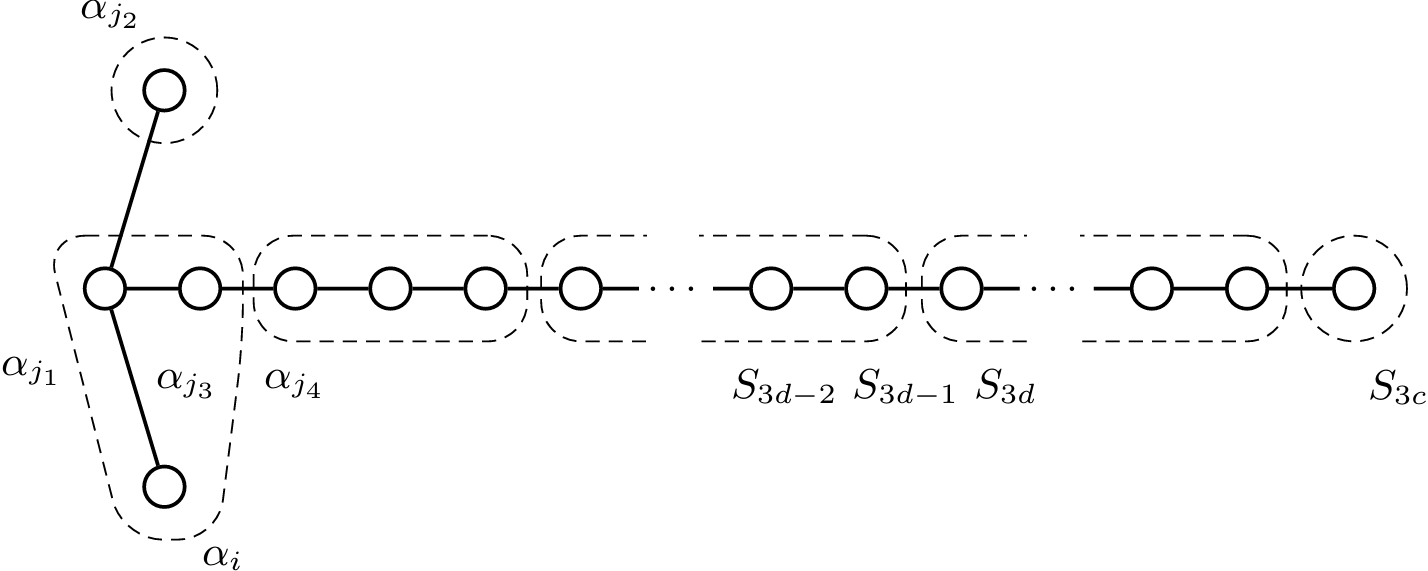
\includegraphics[
            width=2cm,
            height=0.75cm,
            keepaspectratio
        ]{structure/figures_dataset/structure_2.png}
    \end{minipage}
};

\draw[pipelinearrow]
    (simmatrix.north)
    -- (retainedpair.south);

\node[
    llm,
    right=0.35cm of retainedpair,
    yshift=0.11cm,
    minimum width=2cm,
    minimum height=0.7cm
] (vlmblock) {%
    \begin{minipage}{2.1cm}
    \small
        \textbf{VLM Editing}\\
        \tiny
        Analyze differences between Image X + TikZ X and Image Y + TikZ Y...
    \end{minipage}
};

\node[
    anchor=north east,
    inner sep=0pt
] at ($(vlmblock.north east)+(-0.02cm,-0.04cm)$) {%
    
\includegraphics[width=0.38cm]{structure/logos/ai-assistant.png}
};

\draw[pipelinearrow]
    (retainedpair.east)
    -- (vlmblock.west |- retainedpair.east);

\node[
    below=0.35cm of vlmblock,
    inner sep=0pt,
    outer sep=0pt,
    draw=none,
    fill=none,
    align=center
] (instructionblock) {%
    {
    \setlength{\tabcolsep}{0.08cm}
    \begin{tabular}{
        @{}
        p{1.25cm}
        @{\hspace{0.08cm}
        }
        p{1.25cm}
        @{}
    }
    \specialrule{0.55pt}{0pt}{-0.4em}
    \centering
    \fontsize{4.2}{4.5}\selectfont
    \textbf{Forward}\\[-0.5em]
    \rule{1.0cm}{0.4pt}\\[0.12em]

    \raggedright
    \fontsize{2.9}{3.2}\selectfont
    ``Delete the continuation to the right of the node labeled
    \smathn{S_{3c}}: remove the adjacent node labeled
    \smathn{\alpha_{w_1}}, the following horizontal ellipsis, the upper
    node labeled \smathn{\alpha_{z_3}}...''
    
    \vspace{0.2em}
    \textbullet\ Delete node labels\\
    \textbullet\ Regroup dashed regions\\
    \textbullet\ Shift annotations

    &
    
    \centering
    \fontsize{4.2}{4.5}\selectfont
    \textbf{Backward}\\[-0.5em]
    \rule{1.0cm}{0.4pt}\\[0.12em]

    \raggedright
    \fontsize{2.9}{3.2}\selectfont
    ``Extend the horizontal chain to the right of \smathn{S_{3c}} by
    adding a new adjacent node labeled \smathn{\alpha_{w_1}}, followed
    by a horizontal ellipsis. Add an upper node labeled \smathn{\alpha_{z_3}}...''
    
    \vspace{0.2em}
    \textbullet\ Add node labels\\
    \textbullet\ Regroup dashed regions\\
    \textbullet\ Shift annotations

    \end{tabular}
    }
};

\draw[pipelinearrow]
    (vlmblock.south)
    -- ++(0,-0.35cm);

\node[
    inner sep=5pt,
    fit=(arxiv)
        (github)
        (tex)
        (filter)
        (pathone)
        (pathtwo)
        (heatmap)
        (verticalchart)
        (encoder)
        (embmatrix)
        (simmatrix)
        (retainedpair)
        (vlmblock)
        (instructionblock)
] (pipelinebounds) {};

\begin{scope}[on background layer]
\node[
    draw=gray!65,
    dashed,
    rounded corners=4pt,
    fill=gray!5,
    line width=0.3pt,
    inner sep=0pt,
    fit={
        ($(pipelinebounds.north west)+(0.05cm,-0.05cm)$)
        ($(pipelinebounds.south east)+(-0.25cm,0.10cm)$)
    }
] (pipelinebox) {};
\end{scope}

\end{tikzpicture}
\end{adjustbox}

\caption{Construction pipeline for DaEdiTikZ. Scientific figures are collected and standardized, grouped by their scientific context, embedded with a scientific image encoder, paired according to cosine similarity, and passed to a VLM to produce bidirectional editing instructions.}
\label{fig:daeditikz-construction}
\end{figure*}

\paragraph{Dataset Quality Analysis}
To validate instruction inference, two annotators evaluate 125 revision pairs, including 35 overlapping samples for agreement (Figure~\ref{fig:annotation_analysis}). They identify edit plausibility, omissions, hallucinations, and attribute, numeric, or spatial misinterpretations ($\kappa=0.82$), and rate overall quality on a 1--5 Likert scale (weighted $\kappa=0.79$). Overall, 98\% of retained transformations are plausible and 82.9\% of instructions are rated good (4) or very good (5). While 50\% contain at least one error, these are predominantly omissions (34\%) and misinterpretations (33\%), whereas hallucinations are rare (10\%). To quantify the benefit of code grounding, we repeat the analysis without TikZ code on 90 annotations. The error rate increases from 50\% to 80\%, with omissions increasing by 16 percentage points and numeric misinterpretations from 1\% to 8.5\%, indicating that code provides complementary grounding.

\begin{figure*}[t]
\centering
    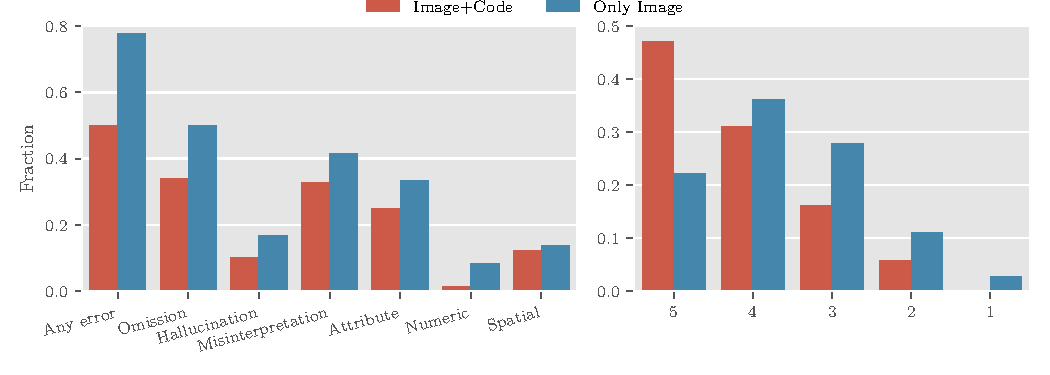
\includegraphics[width=\linewidth]{structure/figures/variant_comparison.pdf}
\caption{Human evaluation of inferred edit instructions. Left: error rates with and without TikZ-code grounding, decomposed into omissions, hallucinations, and attribute, numeric, and spatial misinterpretations. Right: overall instruction quality rated on a 1--5 Likert scale.}
\label{fig:annotation_analysis}
\end{figure*}

\paragraph{DaEdiTikZ-Bench}
To reduce data contamination, we construct DaEdiTikZ-Bench from arXiv submissions published between March and June 2026. For diversity, one pair per submission is retained with 100 pairs sampled from each similarity interval (0.95--0.96, ..., 0.99--1.00), and 50 pairs spanning group sizes from one to ten. We manually inspect all 500 candidates and remove quality issues, trivial edits, and rendering artifacts, leaving 345 revision pairs and 690 editing instances. Six annotators manually correct every VLM-generated instruction by removing hallucinations, correcting misinterpretations, and adding omissions (Figure~\ref{fig:instruction-annotation-pipeline}).

\newlength{\pipelinerowheight}
\setlength{\pipelinerowheight}{1.60cm}

\newcommand{\figimg}[1]{%
  \parbox[c][\pipelinerowheight][c]{1.78cm}{%
    \centering
    \includegraphics[
      width=1.72cm,
      height=1.48cm,
      keepaspectratio
    ]{#1}%
  }%
}

\newcommand{\instructioncell}[1]{%
  \parbox[t][\pipelinerowheight][t]{3.72cm}{%
    \vspace{-7.3pt}%
    \hspace*{0.4mm}%
    \parbox[t]{3.59cm}{%
      \raggedright
      \fontsize{3.15}{3.45}\selectfont
      #1\par
    }%
  }%
}

\begin{figure*}[t]
\centering

\begin{adjustbox}{width=\textwidth}
\begin{tikzpicture}[
    stage/.style={
        draw,
        line width=0.55pt,
        inner sep=0pt,
        outer sep=0pt,
        anchor=north west
    },
    pipeline arrow/.style={
        -{Latex[length=2.2mm,width=1.6mm]},
        line width=0.65pt
    }
]

\node[stage] (pairs) {%
\begin{tabular}{
    @{}
    >{\centering\arraybackslash}p{1.78cm}
    @{\hspace{0.25mm}}
    >{\centering\arraybackslash}p{1.78cm}
    @{}
}
\multicolumn{2}{c}{%
    \parbox[c][0.42cm][c]{3.56cm}{%
        \centering\bfseries\small Image Pair
    }%
}
\\[-0.4mm]
\midrule
\figimg{structure/benchmark_examples/sample_0281_1.png}
&
\figimg{structure/benchmark_examples/sample_0281_2.png}
\\[-0.3mm]
\midrule
\figimg{structure/benchmark_examples/sample_0296_1.png}
&
\figimg{structure/benchmark_examples/sample_0296_2.png}
\\
\end{tabular}
};

\coordinate (pairsepTop) at ($(pairs.north)+(-0.0,-0.46cm)$);
\coordinate (pairsepMidTop) at ($(pairs.north)+(-0.0,-1.9cm)$);
\coordinate (pairsepMidBottom) at ($(pairs.north)+(-0.0,-2.04cm)$);
\coordinate (pairsepBottom) at ($(pairs.south)+(-0.0,0.07cm)$);

\draw[line width=0.35pt]
    (pairsepTop)
    --
    (pairsepMidTop);

\draw[line width=0.35pt]
    (pairsepMidBottom)
    --
    (pairsepBottom);

\node[
    stage,
    right=7mm of pairs.north east,
    anchor=north west
] (generated) {%
\begin{tabular}{@{}p{3.65cm}@{}}
\parbox[c][0.42cm][c]{3.65cm}{%
    \centering\bfseries\small VLM Edit Instruction
}
\\[-0.4mm]
\midrule
\instructioncell{The four boundary lines \smath{\Sigma} are changed from a rotated, intersecting configuration to an orthogonal grid. The lines are now strictly horizontal and vertical, forming a rectangular frame around the center. \redstrike{The central shaded} \redstrike{region labeled \smath{O} is changed from a triangle to a rectangle aligned with the new} \redstrike{grid.} A new label \smath{\Sigma^{4}} is added \redstrike{to the bottom-left quadrant}. A new label \smath{\Theta^{4,1}} is added in the bottom-right corner, marking the angle between the bottom and right boundaries. A new label \smath{\Theta^{3,4}} is added in the bottom-left corner, marking the angle between the left and bottom boundaries. Two new coordinate labels, \smath{x^{4}_{1}} and \smath{x^{4}_{2}}, are added \redstrike{in the bottom quadrant}. The positions of the existing labels
\smath{\Sigma^{1}}, \smath{\Sigma^{2}}, \smath{\Sigma^{3}}, \smath{\Theta^{1,2}}, \smath{\Theta^{2,3}}, and \smath{\Theta^{3,1}} are adjusted to the new geometry.}
\\[-2.9mm]
\midrule
\instructioncell{A new black dot labeled \smath{-Mu} is added to the left of the origin \redstrike{on the dashed line}. A new black dot labeled \smath{(M+n)u} is added to the right of the existing \smath{nu} point \redstrike{on the dashed line}. The horizontal dashed line is extended to the left and right \redstrike{to encompass the new points}. Two new dotted lines are added, parallel to the original one, passing through the new points \smath{-Mu} and \smath{(M+n)u}. A new green wavy path is added, starting from the origin and ending at a green dot on the middle dotted line. The existing blue wavy path is extended further to the right, and its endpoint (blue dot) is moved to a new position on the middle dotted line. A new purple wavy path is added, starting from the origin and ending at a purple dot on the \redstrike{leftmost dotted line}.}
\\[-2.9mm]
\end{tabular}
};

\draw[pipeline arrow]
    ($(pairs.east)$)
    --
    ($(generated.west)$);

\node[
    anchor=center,
    inner sep=0pt,
    fill=gray!20
] at ($(generated.north east)+(-0.5mm,-0.5mm)$) {%
    
\includegraphics[
        width=5.8mm,
        height=5.8mm,
        keepaspectratio
    ]{structure/figures/qwen_logo.png}%
};

\node[
    stage,
    right=7mm of generated.north east,
    anchor=north west
] (corrected) {%
\begin{tabular}{@{}p{3.65cm}@{}}
\parbox[c][0.42cm][c]{3.65cm}{%
    \centering\bfseries\small Human Correction
}
\\[-0.4mm]
\midrule
\instructioncell{The four boundary lines \smath{\Sigma} are changed from a rotated, intersecting configuration to an orthogonal grid. The lines are now strictly horizontal and vertical, forming a rectangular frame around the center. A new label \smath{\Sigma^{4}} is added
\greencorr{at the top-left of the bottom-left quadrant}, \blueadd{representing the fourth boundary}. A new label \smath{\Theta^{4,1}} is added in the bottom-right
corner, marking the angle between the bottom and right boundaries. A new label \smath{\Theta^{3,4}} is added in the bottom-left corner, marking the angle between the left and bottom boundaries. Two new coordinate labels,
\smath{x^{4}_{1}}, \blueadd{pointing downward}, and \smath{x^{4}_{2}}, \blueadd{pointing right}, are added \greencorr{in the center of the bottom quadrant} \blueadd{and associated with the fourth boundary}.}
\\[-2.9mm]
\midrule
\instructioncell{A new black dot labeled \smath{-Mu} is added to the left of the origin \greencorr{just below the dashed line}. A new black dot labeled \smath{(M+n)u} is added to the right of the existing \smath{nu} point. The horizontal dashed line is extended to the left and right. Two new dotted lines are added, parallel to the original one, passing through the new points \smath{-Mu} and \smath{(M+n)u}. A new green wavy path is added, starting from the origin, \blueadd{curving slightly downwards}, and ending at a green dot on the middle dotted line. The existing blue wavy path is extended further to the right,
\blueadd{now curving just over the new rightmost dashed line}. Its endpoint (blue dot) is moved to a new position on the middle dotted line \blueadd{just below the green dot}. A new purple wavy path is added, starting from the origin, \blueadd{curving over the leftmost dotted line}, and ending at a purple dot on the \greencorr{middle dotted line} \blueadd{just below the blue dot}.}
\\[-2.9mm]
\end{tabular}
};

\draw[pipeline arrow]
    ($(generated.east)$)
    --
    ($(corrected.west)$);

\node[
    anchor=north east,
    inner sep=0pt,
    fill=gray!20
] at ($(corrected.north east)+(2.4mm,2.4mm)$) {%
    
\includegraphics[
        width=5.8mm,
        height=5.8mm,
        keepaspectratio
    ]{structure/figures/user-edit.png}%
};

\end{tikzpicture}
\end{adjustbox}

\caption{Examples of human-refined benchmark instructions. \redstrike{Red strikethrough} marks removed errors, \greencorr{green} marks corrections, and \blueadd{blue} marks added omissions.}
\label{fig:instruction-annotation-pipeline}

\end{figure*}